\let\negmedspace\undefined
\let\negthickspace\undefined
\documentclass[journal,12pt,onecolumn]{IEEEtran}
\usepackage{cite}
\usepackage{amsmath,amssymb,amsfonts,amsthm}
\usepackage{amsmath}
\usepackage{algorithmic}
\usepackage{graphicx}
\usepackage{textcomp}
\usepackage{xcolor}
\usepackage{txfonts}
\usepackage{listings}
\usepackage{multicol}
\usepackage{enumitem}
\usepackage{mathtools}
\usepackage{gensymb}
\usepackage{comment}
\usepackage[breaklinks=true]{hyperref}
\usepackage{tkz-euclide} 
\usepackage{listings}
\usepackage{gvv}                                        
\usepackage[latin1]{inputenc}                                
\usepackage{color}                                            
\usepackage{array}                                            
\usepackage{longtable}                                       
\usepackage{calc}                                             
\usepackage{multirow}                                         
\usepackage{hhline}                                           
\usepackage{ifthen}                                           
\usepackage{lscape}
\usepackage{tabularx}
\usepackage{array}
\usepackage{float}


\newtheorem{theorem}{Theorem}[section]
\newtheorem{problem}{Problem}
\newtheorem{proposition}{Proposition}[section]
\newtheorem{lemma}{Lemma}[section]
\newtheorem{corollary}[theorem]{Corollary}
\newtheorem{example}{Example}[section]
\newtheorem{definition}[problem]{Definition}
\newcommand{\BEQA}{\begin{eqnarray}}
\newcommand{\EEQA}{\end{eqnarray}}
\newcommand{\define}{\stackrel{\triangle}{=}}
\theoremstyle{remark}
\newtheorem{rem}{Remark}

\begin{document}
\bibliographystyle{IEEEtran}
\vspace{3cm}

\title{2020-Jan-8-S1}
\author{EE24BTECH11001 -  ADITYA TRIPATHY}
\maketitle

\renewcommand{\thefigure}{\theenumi}
\renewcommand{\thetable}{\theenumi}

\begin{enumerate}
	\item[16.] 
		Let two points be A$\brak{1, -1}$ and B$\brak{0, 2}$. If a point P$\brak{x', y'}$ be
		such that area of $\Delta PAB = 5$sq. units and it lies if the line, $3x + y - 4\lambda = 0,$ then
		the value of $\lambda$ is :
		\hfill{\brak{2020-Jan-8-S1}}
	\begin{multicols}{4}
		\begin{enumerate}
			\item 4 
			\columnbreak
			\item 1
			\columnbreak
			\item -3
			\columnbreak
			\item 3
		\end{enumerate}
	\end{multicols}

	\item[17.] The shortest distance between the lines
		\begin{align*}
		\frac{x-3}{3} = \frac{y-8}{-1} = \frac{z-3}{-1}
		\end{align*} And
		\begin{align}
			\frac{x+3}{3} = \frac{y+7}{2} = \frac{z-6}{1}
		\end{align}
		\hfill{\brak{2020-Jan-8-S1}}
	\begin{multicols}{4}
		\begin{enumerate}
			\item $2\sqrt{30}$ \columnbreak
			\item $\frac{7\sqrt{30}}{2}$ \columnbreak
			\item 3 \columnbreak
			\item $3\sqrt{30}$
		\end{enumerate}
	\end{multicols}


\item[18.] Let the line $y = mx$ and the ellipse $2x^2 + y^2 = 1$ intersect a point $P$ in the first quadrant. If the 
	normal to this ellipse at $P$ meets the co-ordinate axes at $\brak{\frac{-1}{3\sqrt{2}}, 0}$ and $\brak{0, \beta}$
	, then $\beta$ is equal to 
		\hfill{\brak{2020-Jan-8-S1}}
		\begin{enumerate}
			\begin{multicols}{2}
			\item $\frac{2}{\sqrt{3}}$ \columnbreak
			\item $\frac{2}{3}$
			\end{multicols}
			\begin{multicols}{2}
			\item $\frac{2\sqrt{2}}{3}$ \columnbreak
			\item $\frac{\sqrt{2}}{3}$
			\end{multicols}
		\end{enumerate}
		\begin{figure}
			\centering
		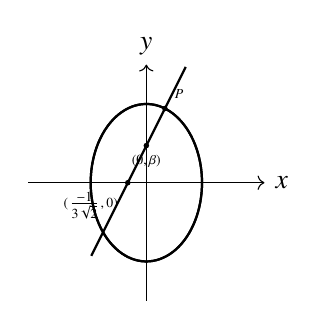
\begin{tikzpicture}
    			\draw[black, thick, domain=0:360, samples=100] 
        			plot ({sqrt(1/2)*cos(\x)}, {sin(\x)}); 
    			\draw[black, thick, domain=0:360, samples=100] 
        			plot ({sqrt(1/2)*cos(\x)}, {-sin(\x)}); 
    
    			\draw[->] (-1.5, 0) -- (1.5, 0) node[right] {$x$};
    			\draw[->] (0, -1.5) -- (0, 1.5) node[above] {$y$};
    
    
    			\draw[black, thick, domain=-0.7:0.5, samples=100]
        			plot ({\x}, {2*(\x) + 0.4714});
    
    			\fill[black] (0, 0.4714) circle (1pt) node[below] {\tiny $(0, \beta)$};
    			\fill[black] ({-1/(3*sqrt(2))}, 0) circle (1pt) node[below left] {\tiny $(\frac{-1}{3\sqrt{2}}, 0)$};
    			\fill[black] (0.235, 0.942) circle (1pt) node[above right] {\tiny $P$};		
		\end{tikzpicture}
		\end{figure}
	\item[19.] If $c$ is a point at which Rolle's Theorem holds for the function,
		\begin{align}
			f(x) = \log_e \brak{\frac{x^2 + \alpha}{7x}}
		\end{align}
		in the interval $\brak{3, 4}$, where $\alpha \in R$, then $f''(c)$ is equal to : 

		\hfill{\brak{2020-Jan-8-S1}}
		\begin{enumerate}
			\begin{multicols}{4}
				\item $\frac{-1}{24}$ \columnbreak
				\item $\frac{-1}{12}$ \columnbreak
				\item $\frac{\sqrt{3}}{7}$ \columnbreak
				\item $\frac{1}{12}$
			\end{multicols}
		\end{enumerate}

	\item[20.] Let
		\begin{align}
			f\brak{x} = x \cos ^{-1}\brak{\sin \brak{-|x|}}, x \in \brak{\frac{-\pi}{2}, \frac{\pi}{2}}
		\end{align}, then which of the following is true
		
		\hfill{\brak{2020-Jan-8-S1}}
		\begin{enumerate}
			\item $f\brak{0} = \frac{-\pi}{2}$ 
			\item $f'$ is decreasing in $\brak{\frac{-\pi}{2}, 0}$ and increasing in $\brak{0, \frac{\pi}{2}}$ 
			\item $f$ is not differentiable at $x = 0$  
			\item $f'$ is increasing in $\brak{\frac{-\pi}{2}, 0}$ and decreasing in $\brak{0, \frac{\pi}{2}}$
		\end{enumerate}


	\item[21.] An urn contains 5 red marbles, 4 black marbles and 3 white marbles. Then the number of ways in which 4
	marbles can be drawn so that at most three of the are red is.
		\hfill{\brak{2020-Jan-8-S1}}
\\
	\item[22.] Let the normal at a point $P$ on the curve $y^2 - 3x^2 + y + 10 = 0$ intersect the y-axis at 
		$\brak{0, \frac{3}{2}}$. If $m$ is the slope of the tangent at $P$ to the curve, te $\abs{m}$ is equal to
		\hfill{\brak{2020-Jan-8-S1}}
		\begin{figure}[ht]
		\centering
		\begin{tikzpicture}
   			\draw[black, thick] (-5, 0) -- (5, 0) node[right] {$x$};
			\draw[black, thick] (0, -5) -- (0, 5) node[above] {$y$};
			\draw[domain=-3.5:-1.8027757,smooth,variable=\x,black] plot ({\x},{(-1 + sqrt(1 + 12*(\x)^2 - 40))/2});
			\draw[domain=-3.5:-1.8027757,smooth,variable=\x,black] plot ({\x},{(-1 - sqrt(1 + 12*(\x)^2 - 40))/2});
			\draw[domain=1.8027757:3.5,smooth,variable=\x,black] plot ({\x},{(-1 + sqrt(1 + 12*(\x)^2 - 40))/2});
			\draw[domain=1.8027757:3.5,smooth,variable=\x,black] plot ({\x},{(-1 - sqrt(1 + 12*(\x)^2 - 40))/2});
    			\draw[black, thick, domain=0.5:3, samples=100]
				plot ({\x}, {4 * (\x) - 7});
    			\draw[black, thick, domain=-3:6, samples=100]
				plot ({\x}, {-0.25 * (\x) + 1.5});
    			\fill[black] (2, 1) circle (3pt) node[left] {\small $(2, 1)$};
			\fill[black] (0, 1.5) circle (3pt) node[above] {\small $(0, \frac{3}{2})$};
		\end{tikzpicture}
		\end{figure}
\\	
	\item[23.] The least positive value of $'a'$ for which the equation
	\begin{align}
		2x^2 + \brak{a - 10}x + \frac{33}{2} = 2a
	\end{align} has real roots is
		\hfill{\brak{2020-Jan-8-S1}}
\\
	\item[24.] The sum
	\begin{align}
		\sum_{k = 1}^{20} \brak{1 + 2 + 3 + \dots + k}
	\end{align} is
		\hfill{\brak{2020-Jan-8-S1}}
\\
	\item[25.] The number of all 3 $\times$ 3 matrices $A$, with entries from the set $\{-1, 0 , 1\}$, such that the sum
	of the diagonal elements of $\brak{AA^\top}$ is 3, is
		\hfill{\brak{2020-Jan-8-S1}}
	\end{enumerate}
\end{document}
